%------------------------------------------------------------------------------------------------------------------------
% Literature review of recent advances in modeling seismic waves propagation using machine   
% learning-based methods
%------------------------------------------------------------------------------------------------------------------------
% Author: oscar-rincon
% Email: orincon@eafit.edu.co
% Creation date: 2024-03-15
% Version: 1.0
%------------------------------------------------------------------------------------------------------------------------
\documentclass[11pt,twoside]{article}
%------------------------------------------------------------------------------------------------------------------------
% Import the style file
%------------------------------------------------------------------------------------------------------------------------
\usepackage{review_seismic_waves}
%------------------------------------------------------------------------------------------------------------------------
% Document starts here
%------------------------------------------------------------------------------------------------------------------------
\begin{document}

% Set the page style to empty (no headers or footers)
\thispagestyle{empty}  

%------------------------------------------------------------------------------------------------------------------------
% Title, Author, and Affiliation
%------------------------------------------------------------------------------------------------------------------------

% Create a colored box with specific background and frame colors, and sharp corners
%\begin{tcolorbox}[colback=white!20,colframe=gray!20,sharp corners]

% Add vertical space adjustment
\vspace{-2mm} 
% Create a minipage for the title
\begin{minipage}{11.5cm}
    \begin{center}
        % Title of the document
        \textbf{\large A Review of Recent Progress in Seismic Waves Propagation Modeling Using 
        Machine Learning Based Methods}  
    \end{center}                 
\end{minipage} 
% Create a minipage for the first logo
\begin{minipage}{4.2cm}
    \begin{center}
        % Include the first logo with specific width
        \hspace{-0.2cm}
\includegraphics[width=2.8cm]{figs/format/Logo_EAFIT.pdf}
    \end{center}
\end{minipage}    
% Create a minipage for the second logo
% \begin{minipage}{2.2cm}
%     \begin{center}
%         % Include the second logo with specific width
%         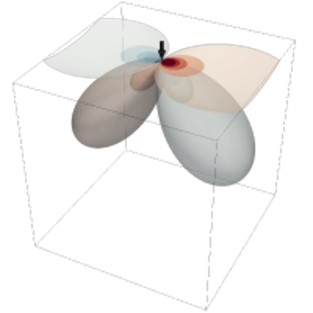
\includegraphics[width=2.5cm]{figs/format/logo_grupo.pdf}
%     \end{center}
% \end{minipage}
% Add vertical space adjustment
\vspace{-2mm} 
%\end{tcolorbox}

% Create another colored box with specific background and frame colors, and sharp corners
%\begin{tcolorbox}[colback=white!20,colframe=gray!20,sharp corners]

% Author's name with ORCID and GitHub links
{\begin{center}
Oscar Rincón-Cardeño\textsuperscript{1, 2,*,\href{https://orcid.org/0000-0002-5308-9710}{\aiOrcid},
\href{https://github.com/oscar-rincon}{\faGithubSquare}}
\end{center}
}

% Add vertical space adjustment
\vspace{-0.3cm}

% Author's affiliations
{\footnotesize
\noindent\textsuperscript{1} School of Applied Sciences and Engineering, Universidad EAFIT, 
Medellín, Colombia\\
\noindent\textsuperscript{2} Applied Mechanics Research Group from Universidad EAFIT\\
\noindent\textsuperscript{*} Correspondence: orincon@eafit.edu.co
}

%------------------------------------------------------------------------------------------------------------------------
% Associated document repository link
%------------------------------------------------------------------------------------------------------------------------

{\noindent\footnotesize{\href{https://github.com/oscar-rincon/review-seismic-waves}
{\faGithubSquare \href{https://github.com/oscar-rincon/review-seismic-waves}{ https://github.com/oscar-rincon/review-seismic-waves}}
}
}

%\end{tcolorbox}

%------------------------------------------------------------------------------------------------------------------------
% Abstract of the document
%------------------------------------------------------------------------------------------------------------------------

% Create a colored box with specific background and frame colors, and sharp corners
\begin{tcolorbox}[colback=gray!20, colframe=gray!20, sharp corners]

    % Begin the abstract section
    \begin{abstract}

        % Add vertical space adjustment
        \vspace{-1mm}

        % No indentation for the first paragraph
        \noindent
        % Abstract content      
        Numerical modeling has been crucial for addressing problems across various scientific and engineering 
        disciplines involving partial differential equations. In particular, wave propagation modeling has seen
         significant development in scientific computation. Standard numerical modeling methods have demonstrated 
         notable accuracy; however, their computational cost can be substantial. Recently, alternative methods based 
         on machine learning have emerged, offering a promising balance between computational cost and accuracy 
        when applied to wave propagation problems. In this work, we present a review of methods developed and used 
        to model wave propagation, with a special emphasis on computational seismology. We discuss the fundamentals 
        of wave propagation modeling, standard numerical methods, and recent advances in solving differential 
        equations through these approaches. We conduct a systematic review of the literature to identify 
        applications where these methods, either standalone or in hybrid approaches with standard numerical methods, 
        have demonstrated efficiency in terms of computational time. The results of this review provide insights 
        into the potential of machine learning techniques for wave propagation modeling and their impact on 
        computational seismology.        
    \end{abstract}

    \keywords{wave propagation, numerical methods, machine learning, partial differential equations, computational seismology.}   

\end{tcolorbox} 

%------------------------------------------------------------------------------------------------------------------------
% Section - Introduction
%------------------------------------------------------------------------------------------------------------------------ 
\section*{Introduction}
\fancyhead[RO]{\textit{Introduction}\, / \thepage} 
%------------------------------------------------------------------------------------------------------------------------

\lettrine{\textcolor{gray}{W}}{ }ave propagation is a physical phenomenon governed by partial differential equations, 
which hold significant importance across various applied sciences and engineering fields. However, analytical 
solutions are not always available in many practical situations and numerical methods are usually required to 
approximate the exact solutions. Consequently, these methods have been applied to solve the partial differential 
equations \citep{Seriani2020}.

In the field of wave propagation, numerous techniques address wave propagation challenges. Classical methods include 
finite-difference, finite-element and spectral-element methods \citep{Moczo, virieux_review_2011, Igel2017,
komatitsch_introduction_1999,chaljub_spectral-element_2007}. In these approaches, the spatial coordinates are discretized. 
In the context of mathematical modeling, the primary objective is to ensure that the solution methods 
are computationally efficient without sacrificing accuracy to capture the physical details inherent to the 
system. However, standard numerical methods often encounter difficulties when addressing complex problems 
such as irregular geometries, material changes, and mixed boundary conditions. Therefore, the computational 
demand associated with many common models in computer sciences and engineering has increased the development 
of innovative strategies.

Research conducted with the use of machine learning has considerably grown in the late 2010s, owing to advancements 
in hardware, such as graphic processing units and data storage technologies and the growth of available data. 
Additionally, the discovery of better training practices for neural networks, and the availability of open-source 
packages like Tensorflow, PyTorch and JAX \citep{abadi_tensorflow_2016,paszke_pytorch_2019,jax2018github}, as well 
as the availability of Automatic Differentiation in such packages \citep{paszke_automatic_2017,baydin_automatic_2017}. 
Particularly, neural networks learning algorithms offer attractive approximation capabilities for any function by 
mapping the input features to the output targets in a data-driven manner. A version of the Universal Approximation 
Theorem conclusively demonstrates that neural networks have the capability to accurately approximate a wide 
variety of nonlinear functions without any dimensionality constraints \citep{barron_universal_1993}. Therefore 
computational scientists have explored the potential of machine learning to model systems governed 
by partial differential equations \citep{cuomo_scientific_2022,karniadakis_physics-informed_2021}. From those
works, physics-informed neural networks is one of the methods that has gained more attention in the last years,
cited by over 10,000 publications \citep{Raissi2019}. Figure \ref{fig:publications_absolute_relative} shows the 
number of document published associated to wave propagation modeling and machine learning. 


\begin{figure}[H]
\centering
    
\includegraphics[width=1.0\textwidth]{figs/publications_abs_relat.pdf}
    \caption{The growth of literature related to machine learning and wave propagation modeling. Number of publications 
    according to Scopus between 2010 and 2023. The implemented query was: "machine learning" OR "deep learning" 
    OR "neural networks" AND "wave propagation" OR "wave equation" AND (modeling OR modelling OR model OR simulation) 
    AND (PUBYEAR > 2009 AND PUBYEAR < 2024). The relative number of publications is calculated as the number of
    publications with the choosen terms with respect to the total number of publications in Scopus between 2010 and 2023.
    The absolute number of publications is shown in red, and the relative number of publications is shown in blue.} 
    \label{fig:publications_absolute_relative}
\end{figure}


Remarkable reviews have been conducted to address the increasing use of machine learning algorithms across various 
engineering and scientific disciplines \citep{vadyala_review_2022,deng_physics-informed_2023,lino_current_2023}. 
Also emphasis has been placed on the application of neural networks in the field of computational seismology 
\citep{jingbo_research_2023}. However, there is uncertainty, given the rapid growth of the field, about in which 
cases machine learning methods can be an appropriate alternative to standard numerical methods to solve partial 
differential equations \citep{grossmann_can_2023,mcgreivy_weak_2024}. Although in principle, machine learning 
methods have the potential to learn a surrogate model able to approximate the solution of a partial differential 
equation, some methods can be more efficient than others according to the problem being solved. This is 
particularly relevant in the context of computational seismology, where the complexity of the domain phenomena can 
be challenging to model. Therefore the aim of this review is to provide insights into the potential of machine 
learning methods for wave propagation modeling and their impact on computational seismology.

This work provides a comprehensive analysis of the advancements made in partial differential equations modeling 
through machine learning and their impact. While this area can be applied to a wide range of problems, our focus 
will be limited to the propagation of seismic waves. The work is organized into the following sections: Section 
\ref{sec:modeling_wave_propagation} describes general aspects about wave propagation modeling. Furthermore, 
in Sections \ref{sec:standard_numerical_methods} and \ref{sec:machine_learning_methods}, we identify 
existing standard and machine learning methods used to solve the diferential equations and with particular emphasis 
on the wave equation. Then, in Section \ref{sec:applications} we systematically review the recent advances in wave 
propagation modeling achieved through these emerging methods and identify when they can be an alternative to 
traditional numerical methods or in an hibrid way when they can improve the solver performance in terms of 
computational time. This review may be of help for researchers with interest into apply 
these emerging techniques in wave propagation modeling. Due to the extensive areas where machine learning is 
applied, our aim is to identified the potential of these methods in computational seismology.

%------------------------------------------------------------------------------------------------------------------------
% Section - 1 - Modeling of Wave Propagation
%------------------------------------------------------------------------------------------------------------------------
\section{Modeling of Wave Propagation}\label{sec:modeling_wave_propagation}
\fancyhead[RO]{\textit{Modeling of Wave Propagation}\, / \thepage} 
%------------------------------------------------------------------------------------------------------------------------

A dynamic model, such as the propagation of waves in a medium, describes how a system changes over time. This is 
different from a static model, which shows how a system is at equilibrium. Dynamic models typically use differential 
equations to describe how a system evolves. A general formulation of the governing equation of a physical problem can be:

\begin{equation*}
D(u(x,t); \lambda) = f(x,t), \quad x \in \Omega, \quad t \in [0, T]\label{eq:pde}
\end{equation*}
 
where $D$ denotes the differential operator acting on the solution to the differential equation $u(x,t)$ parameterized 
by $\lambda$ and $f(x, t)$ is a source term. While, $\Omega$ and $\partial\Omega$ denote the spatial domain and its boundary. 
Equation \ref{eq:pde} can be used to model different systems. We denote the corresponding boundary conditions and the 
initial condition by:

\begin{equation*}
B (u(x, t)) = g(x, t), \quad x \in \partial \Omega, \quad t \in [0, T] 
\end{equation*}

and

\begin{equation*}
u(x, 0) = h(x, 0), \quad x \in \Omega
\end{equation*}

The prescribed initial condition and boundary condition are characterized via $h(x)$ and $g(x, t)$. Two general approaches 
when mathematically modeling a system are the inverse and forward problems. The process of determining the causes 
of a set of observations is known as the inverse problem \citep{Tarantola}, aiming to infer, for example, the properties of a 
medium based on its reaction to wave propagation. Since it begins with the effects and then calculates the causes, it is the 
opposite of a forward problem, which determines the effects based on the causes. In most cases, the inverse problem is formulated 
by iteratively performing forward modeling to infer the causes that produce a desired effect, making it computationally complex. 
An schematic representation of the forward and inverse model using numerical methods is shown in Figure \ref{fig:forward_inverse}.

\begin{figure}[h]
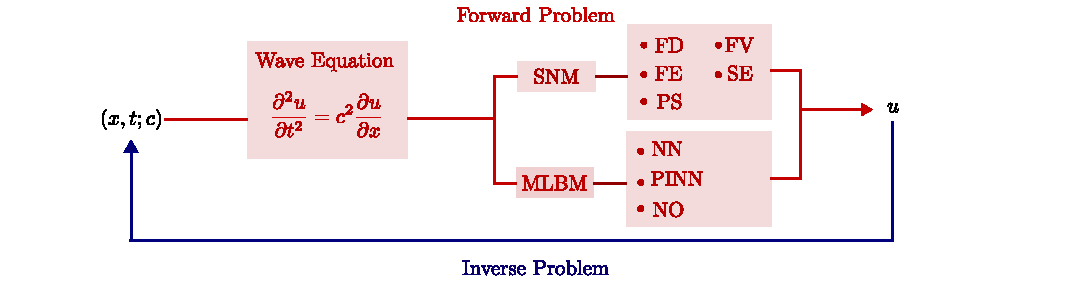
\includegraphics{figs/forward_inverse_modeling_waves.pdf}
    \caption{Scheme of the forward and inverse problems encountered in solving partial differential equations. In the forward 
    scenario, the inputs $(x,t;c)$ are employed to characterize a model across PDEs. Subsequently, the PDEs are resolved through 
    either standard numerical methods (SNM) or neural networks based methods (MLBM) to derive a solution $u$. Standard numerical 
    methods such as: finite differences (FD), finite elements (FE), pseudo-spectral (PS), finite volumes (FV), and spectral 
    elements (SE). Also, deep learning techniques include, for example, Physics Informed Neural Networks (PINNs), Neural Operator 
    (NO), and Neural Networks (NN). In the case of the inverse problem, the objective is to determine the parameters, for example, 
    the wave speed, $c$ starting from the solution $u$.}
    \label{fig:forward_inverse}
\end{figure}

Inverse problems are closely tied to simulation, and solving them is crucial for many real-world tasks. Moreover, some complex 
physical problems require determining the properties of a physical system governed by partial differential equations from 
observational data, rather than solving them directly to obtain a function that satisfies them 
\citep{galiounas_battery_2022, ren_seismicnet_2024,mccann_convolutional_2017}. The objective is to estimate a set of latent or 
unobserved parameters of a system based on real-world observations. Within the framework described by Equation \ref{eq:pde}, 
the task involves estimating $\lambda$ given $u$. Inversion can be exceedingly challenging since often requires numerous forward 
simulations to align the predictions of the physical model with the set of observations. 

Despite being the most elementary among mechanical wave equations, the scalar (acoustic) wave equation is widely used to study 
seismic waves and in medical applications \citep{moseley_physics-informed_2022, alkhadhr_wave_2023}. The second-order linear 
wave equation in a homogeneous medium can be expressed as \citep{Carcione2002}:

\begin{equation*}
\frac{\partial^2 u(x_i, t)}{\partial t^2} - c^{2} \nabla^2 u(x_i, t) = f(x_i, t) \ ,
\label{acoustic}
\end{equation*}

where \( u(x_i, t) \) describes the pressure of the generated seismic waves, and \( f(x_i, t) \) is a source term that 
describes the strength and duration of the source.

Another common expression used to describe the propagation of seismic waves, for the case of a heterogeneous 
isotropic medium, is the elastic wave equation \citep{moseley_fast_2018, lehmann_fourier_2023}. This equation can 
be expressed as:

\begin{equation*}
\rho \frac{\partial^2 u}{\partial t^2} = \nabla (\lambda (\nabla \cdot u)) + \nabla \mu \left[\nabla u 
+ (\nabla u)^T\right] + (\lambda + 2\mu) \nabla (\nabla \cdot u) - \mu \nabla \times (\nabla \times u) \ ,
\label{elastic}
\end{equation*}

where $\rho$ is the material density, $u$ is the displacement vector, and $\lambda$, $\mu$ are the Lamé parameters 
characterizing the material. These equations are fundamental for modeling the propagation of seismic waves in 
elastic media. The acoustic wave equation is a simplification that assumes the waves are longitudinal and the 
medium is homogeneous and isotropic. In contrast, the elastic wave equation accounts for the heterogeneous 
and anisotropic properties of the medium, allowing for the modeling of both longitudinal and transverse waves.

Besides the acoustic and elastic equations, there are other important variants of the wave equation used in different 
contexts of computational seismology. Viscoelastic Wave Equation is a variant tha incorporates damping effects due to 
the viscosity of the medium. It is useful for modeling wave attenuation in real geological media that exhibit 
viscoelastic behavior.

\begin{equation*}
\rho \frac{\partial^2 u}{\partial t^2} = \nabla (\lambda (\nabla \cdot u)) + \nabla \mu \left[\nabla u + 
(\nabla u)^T\right] + (\lambda + 2\mu) \nabla (\nabla \cdot u) - \mu \nabla \times (\nabla \times u) - 
\eta \frac{\partial u}{\partial t} \ ,
\label{viscoelastic}
\end{equation*}
    
where $\eta$ is the viscosity coefficient. Anisotropic Wave Equation describe propagation in anisotropic media, 
the elastic properties vary with direction. The wave equation is modified to include additional terms representing 
this anisotropy.

\begin{equation*}
\rho \frac{\partial^2 u}{\partial t^2} = \nabla \cdot \sigma + f \ ,
\label{anisotropic}
\end{equation*}
    
where $\sigma$ is the anisotropic stress tensor and $f$ is a source term. Nonlinear Wave Equation are considered 
in situations where wave amplitudes are very large, linear approximations are insufficient, and nonlinear terms 
must be considered in the wave equation.

\begin{equation*}
\frac{\partial^2 u}{\partial t^2} - c^2 \nabla^2 u + \beta \frac{\partial u^2}{\partial x^2} = f(x_i, t) \ ,
\label{nonlinear}
\end{equation*}
    
where $\beta$ is a nonlinearity coefficient. These variants allow for more precise and realistic modeling 
of seismic wave propagation in different types of media and under various conditions. The choice of the 
appropriate wave equation depends on the characteristics of the medium and the seismic phenomenon being studied. 
Tradicionally, the wave equation and its applications to computational seismology have been solved using standard 
numerical methods \citep{Igel2017}.

%------------------------------------------------------------------------------------------------------------------------
% Section - 2 - Standard Numerical Methods 
%------------------------------------------------------------------------------------------------------------------------
\section{Standard Numerical Methods}\label{sec:standard_numerical_methods}
\fancyhead[RO]{\textit{Standard Numerical Methods}\, / \thepage}
%------------------------------------------------------------------------------------------------------------------------

In the past decades various numerical methods have been proposed to solve physics systems by partial differential 
equations such as the wave equation. The finite-difference method is among the most 
popular to solve partial differential equations, and particularly the wave equation. This possibly associated with 
its simplicity and efficiency. A complete review of the finite-differences method applied to wave propagation can be 
found the \citeauthoryear{Moczo2014}. Partial derivatives are approximated by discrete operators involving differences 
between adjacent grid points. The finite difference method suits for tackling issues related to simple geometric 
structures. In contrast, other methods such as the finite element offers more grid flexibility, facilitating the 
handling of intricate geometric boundaries.

In wave propagation simulations, the partial differential equations are typically discretized on a staggered grid 
\citep{madariaga_dynamics_1976,Virieux1986}. This approach facilitates the resolution of the rupture propagation 
problem. Particularly an approach was proposed in the work of \citeauthoryear{Zhou2021} a finite-difference method 
with variable-length temporal and spatial operators was proposed to increase the stability and efficiency of the 
standard method. Also, \citeauthoryear{liu_simulation_2023} combined a standard staggered-grid, finite-difference 
approach and the perfectly matched layer absorbing boundary to solve 3D first-order velocity-stress equations of 
acoustoelasticity to simulate wave propagating.

Finite-element methods are suitable for dealing with intricate shapes and diverse materials because they can use 
irregular grids. They permit flexibility in size, shape, and approximation order. Nevertheless, a drawback is their 
high demand for computing power. This methodology involves the transformation of the problem at hand into a system 
of linear equations utilizing the weak formulation of the pertinent differential equation. This transformation is 
facilitated by employing an interpolation basis comprised of polynomials defined over disjoint domains, commonly 
referred to as elements.

Open-source software is available for applying numerical methods to solve the wave equation. For example, FEniCS 
and DUNE \citep{FEniCS,sander_dune_2020}, offer computing frameworks designed for solving partial differential 
equations using the finite element method. SPECFEM, which specializes in seismic wave propagation, is widely used 
in simulations implemented in Fortran \citep{dimitri_komatitsch_2023_10415228,komatitsch_2024_10823181}. Similarly, 
SEISMIC\_CPML \citep{komatitsch_unsplit_2007} uses finite differences for modeling. These implementations of 
standard methods have enabled effective simulations of the wave equation.

A significant difficulty in using standard methods for wave propagation simulations is their computational cost. Their 
accuracy is achieved at the expense of the number of points in the grid. Modeling a complex domain can entail a huge 
amount of grid points, with the wavefield requiring iterative updates across the entire grid at each time step. 
Associated with the required discretization is the challenge when dealing with high-dimensional systems. The curse 
of dimensionality can lead to a rapid increase in computational cost as the number of dimensions grows. Additionally, 
model evaluation and storage could be significantly costly \citeauthoryear{saloma_computational_1993}, and their 
limited capacity to incorporate measured data into their predictions makes them less ideal for use in inverse problems. 
There is considerable scientific interest in employing machine learning techniques to address these challenges.

%------------------------------------------------------------------------------------------------------------------------
% Section - 3 - Machine learning Methods 
%------------------------------------------------------------------------------------------------------------------------
\section{Machine learning Methods}\label{sec:machine_learning_methods}
\fancyhead[RO]{\textit{Machine learning Methods}\, / \thepage} 
%------------------------------------------------------------------------------------------------------------------------

The field of machine learning has recently shown significant promise in approximating predictions of physical 
phenomena. These methods are capable of capturing highly nonlinear physics and provide substantially faster inference 
times compared to traditional simulations. Consequently, machine learning has been employed as an alternative to 
conventional methods, leveraging its capability as a universal function approximator \citep{hornik_approximation_1991}.
For example, support vector machines have been used to solve ordinary and partial differential equations. Although 
this method was originally designed for classification tasks, an extention to the method that apply least square to 
the objetive function has been proposed to solve differential equations \citep{mehrkanoon_approximate_2012,
mehrkanoon_learning_2015}.

Neural network based methods are a subset of machine learning, whose models are composed of an artificial neural 
network with a single or multiple processing layers (Figure \ref{deep_learning_subset_architecture}.A). It have 
shown potential in overcoming the limitations of multiple approaches in various fields such as computer vision, 
natural language processing, and genomics \citep{lecun_deep_2015,goodfellow_deep_2016}. The fundamental architecture 
of a neural network architecture is conformed by an input layer, an output layer, and an arbitrary number of hidden 
layers. Particularly, in a fully connected neural network, neurons in adjacent layers are connected with each other 
but neurons within a single layer share no connection (Figure \ref{deep_learning_subset_architecture}.B). Furthermore, 
neural networks methods have emerged as an attractive tool to augment and complement conventional numerical solvers 
of partial differential equations, thereby enabling the tackling of challenges across multiple dimensions, scales, 
and parameterization with the promise of efficiency and precision. 

\begin{figure}[h]
\centering
    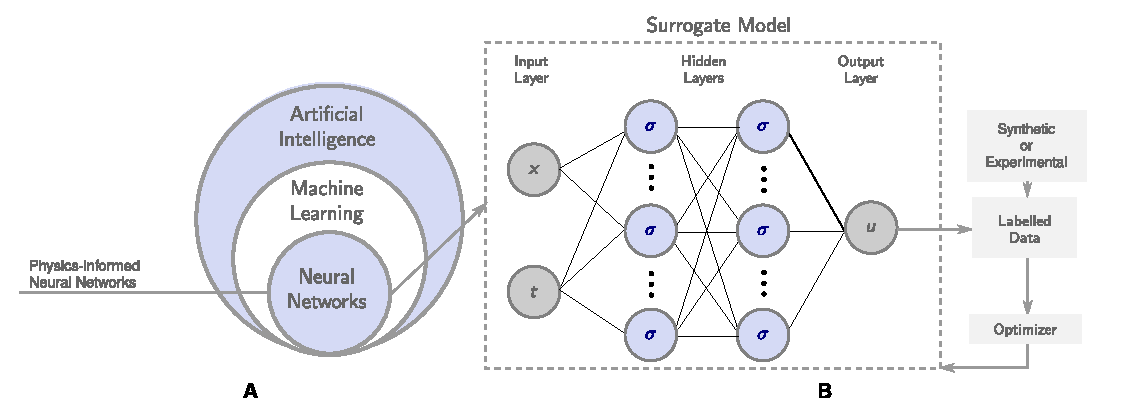
\includegraphics[width=1.0\textwidth]{figs/artificial_intelligence_subsets.pdf}
    \caption{Artificial Intelligence subsets. (A) Deep learning as a subset of machine learning and artificial 
    intelligence and (B) basic architecture of artificial neural networks.}    
    \label{deep_learning_subset_architecture}
\end{figure}

They essentially model the partial differential equation solution by a deep neural network and train the 
network’s parameters to approximate the solution. Data-driven neural networks methods are capable of directly 
learning the trajectory of a system of partial differential equations from available data 
\citep{li_neural_2020,li_fourier_2021}. Alternatively, syntetic data generated by standard numerical 
methods can be used to train the neural network. Therefore, a surrogate model can be used to predict the
solution of the partial differential equation at a reduced computational cost. While keeping an acceptable
level of accuracy.

One of the most popular types of deep neural networks is known as convolutional neural networks. A 
convolutional neural network convolves learned features with input data, and uses 2D convolutional 
layers, making this architecture well suited to processing 2D data, such as images.

All these approaches employ machine learning algorithms and others such as support vector machines, 
random forests, Gaussian processes have been also applied to model physical systems. However, they 
are implemented mainly as black-box tools. The constructed neural network can be thought of being 
ignorant of the mathematical description of the physical phenomenon. In order to overcome this 
limitation physics-informed neural networks architectures have been proposed. Where the activation 
and the loss functions are designed according to the context of the problem.

There has been an increasing interest in leveraging physics-informed neural networks to solve forward and 
inverse problems where full or partial knowledge of the governing equations is known since the published 
works of \citeauthoryear{raissi_hidden_2018}, \citeauthoryear{raissi_numerical_2018} and 
\citeauthoryear{Raissi2019}. Although similar ideas for constraining neural networks using physical 
laws have been explored in previous studies \citep{lagaris_artificial_1998}. The general principle of 
physics-informed neural networks is to integrate deep neural networks and physical laws to learn the 
underlying consistent dynamics from small or zero labeled data \citep{karniadakis_physics-informed_2021}. 
As universal approximators, neural networks have the potential to represent any partial differential 
equation. This capability eliminates the need for the discretization step, thereby avoiding 
discretization-based physics errors as well. 

\begin{figure}[h]
\centering
    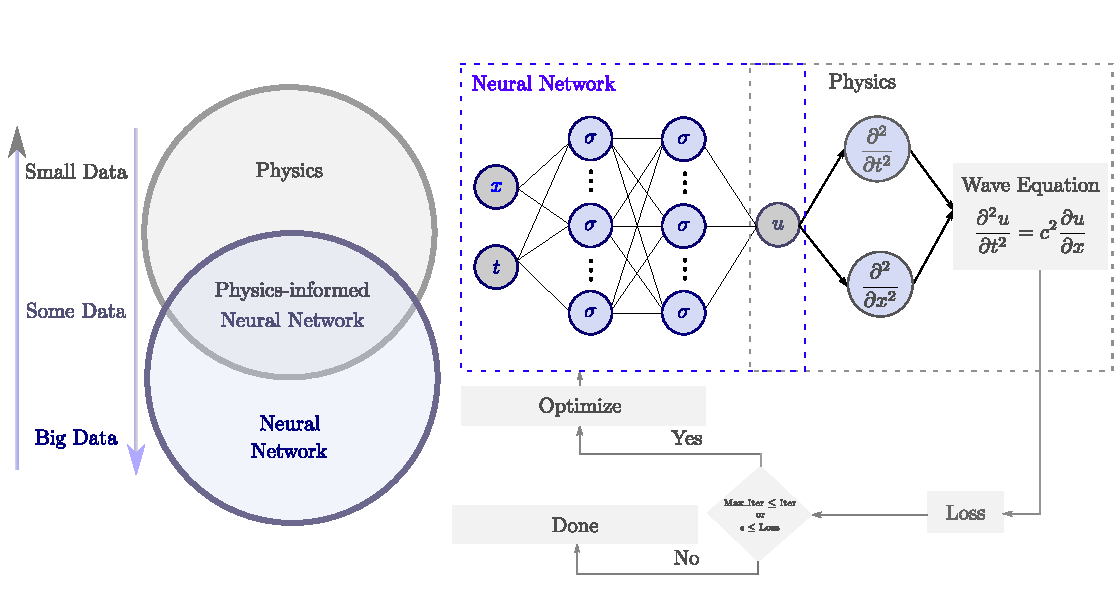
\includegraphics[width=1.0\textwidth]{figs/scheme_pinns_waves.pdf}
    \caption{Physics-informed neural networks scheme applied to the wave equation.}
    \label{deep_learning_subset_architecture}
\end{figure}

Physics-informed neural networks aim to address physical systems governed by the equation

$$
u_{tt} - D[u(t, x); \lambda] = 0,
$$

where \(x \in \mathbb{R}^D\) and \(t \in \mathbb{R}\). The expression \(N[u(t, x); \lambda]\) denotes 
an underlying differential operator that characterizes the physical system, parametrized by \(\lambda\). 
The function \(u(t, x)\) represents the system's solution. The loss function is of the general form 

$$ L := \beta_{\text{pde}}L_{\text{pde}}(\sigma) + \beta_{\text{ic}}(\sigma) L_{\text{ic}} + 
\beta_{\text{bc}} L_{\text{bc}}(\sigma) ,$$

where

$$
\begin{aligned}
& \mathcal{L}_{pde}(\boldsymbol{\sigma})=\frac{1}{n_{pde}} \sum_{i=1}^{n_{pde}}\left|u_{tt} - \mathcal{D}\left[\hat{u}\left(t,
 \boldsymbol{x}_i ; \boldsymbol{\sigma}\right)\right]-f\left(t, \boldsymbol{x}_i\right)\right|^2, \\
& \mathcal{L}_{bc}(\boldsymbol{\sigma})=\frac{1}{n_{bc}} \sum_{i=1}^{n_{bc}}\left|\hat{u}\left(t, \boldsymbol{x}_i ;
 \boldsymbol{\sigma}\right)-g\left(t, \boldsymbol{x}_i\right)\right|^2, \\
& \mathcal{L}_{ic}(\boldsymbol{\sigma})=\frac{1}{n_{ic}} \sum_{i=1}^{n_{ic}}\left|\hat{u}\left(0, \boldsymbol{x}_i ;
 \boldsymbol{\sigma}\right)-h\left(t,\boldsymbol{x}_i\right)\right|^2,
\end{aligned}
$$

and \( L_{\text{pde}} \) represents the residuals of the PDEs, \( L_{\text{ic}} \) represents the error at the collocation points at the 
initial time point, and \( L_{\text{bc}} \) represents the error at the collocation points on the boundaries. The coefficients 
\(\beta_{\text{ic}}\) and \(\beta_{\text{bc}}\) are training hyper-parameters.

One major drawback of these methods is the difficulty of transferring knowledge between different configurations. For example, when solving 
the wave equation, CNNs and PINNs are trained with a fixed velocity parameter and cannot predict anything for a different velocity value. 
One of the main challenges in numerically modeling mechanical is associated with the dimensional, given the computational complexity.

Tackling complex high-dimensional systems comes with significant challenges. Despite this, machine learning-based algorithms offer promising 
prospects for solving partial differential equations, as indicated by studies such as the one by \citeauthoryear{blechschmidt_three_2021}. 
Most of the applications are implemented in one dimensional or two-dimensional domains. In \citeauthoryear{lehmann_fourier_2023} the Fourier 
Neural Operator method is applied to model sesimic waves.

Emerging machine learning methods for solving partial differential equations can face difficulties in establishing fair comparison points 
with standard numerical methods. \citeauthor{mcgreivy_weak_2024} identified two common pitfalls. First, comparing the runtime of a less 
accurate machine learning method to a more accurate standard numerical method, whereas a fair approach would be to make the comparison under 
similar accuracy levels. Second, evaluating the standard numerical method that is not suitable for the partial differential equation being 
solved. These two criteria are essential for properly evaluating performance, but they are not always followed. 
 
Different extentions of the classical work where PINNs was originally proposed have emerged. \citeauthoryear{kharazmi_variational_2019} 
proposed variational physics-informed neural networks which instead trained physics-informed neural networks using the variational form of the 
underlying differential equations. A neural network is still used to approximate the solution of the differential equation, but it is combined 
with a set of analytical test functions to compute the residual of the variational form of the equation in its physics loss term. Furthermore, 
they used quadrature points to estimate the corresponding integrals in the variational loss, rather than random collocation points. They found 
that the variational physics-informed neural networks was able to solve differential equations including Poisson’s equation with similar or 
better accuracy to a physics-informed neural networks trained using the strong form, whilst requiring less collocation points to train. 
However, most of these extensions have not yet been applied to wave propagation modeling.

Various open-source frameworks are available for solving partial differential equations using emerging machine learning methods. Python 
packages such as NeuroDiffEq \citep{chen2020neurodiffeq} and DeepXDE \citep{lu2021deepxde} facilitate the solving of both ordinary and 
partial differential equations using neural networks as function approximators. A similar implementation in the Julia programming language 
is NeuralPDE \citep{https://doi.org/10.48550/arxiv.2107.09443}. Additionally, PINNs-Torch \citep{bafghi_pinns-torch_2023} enables the 
application of Physics-Informed Neural Networks using PyTorch, offering improved performance compared to the original model.

%------------------------------------------------------------------------------------------------------------------------
% Section - 4 - Applications
%------------------------------------------------------------------------------------------------------------------------
\section{Applications}\label{sec:applications}
\fancyhead[RO]{\textit{Applications}\, / \thepage}  
%------------------------------------------------------------------------------------------------------------------------

This section provides a systematic review of the literature on applying machine learning methods to model 
wave propagation. We aimed to answer the following research question:

\begin{quote}
\noindent\textbf{In which computational seismology applications have machine learning methods demonstrated to be 
an appropriate \textit{complement} or \textit{alternative} to standard numerical methods in terms of computational 
time and accuracy?}
\end{quote}

In order to answer this question, we considered works related with the field of interest that offered a comparative 
analysis between machine learning methods and standard numerical methods. In the research question we referred to 
a \textit{complementary} approach when either a mixed method that combines machine learning and standard numerical methods 
or a machine learning method was trained with data generated by a standard numerical method. Additionally, we have 
opened the scope to include works where physics informed neural networks have been applied to solve inverse problems. 
Since, generally, when applied to forward problems, they have shown to be both less accurate and computationally 
inefficient given the required amount of time to train the model. However, when applied to inverse problems, they have 
demostrated to be a promising \textit{alternative} to standard numerical methods 
\citep{haghighat_physics-informed_2021,raissi_hidden_2020}. This given its versatility to 
deal with variable amounts of data and at the same time the ability to incorporate physical laws into the model.  

A search strategy was implemented to identify relevant publications that allow a comparison between machine 
learning methods and standard numerical methods in the context of wave propagation. The flowchart and total 
number of works that met these conditions are shown in Figure \ref{fig:scheme_systematic_review}.

\begin{figure}[h]
    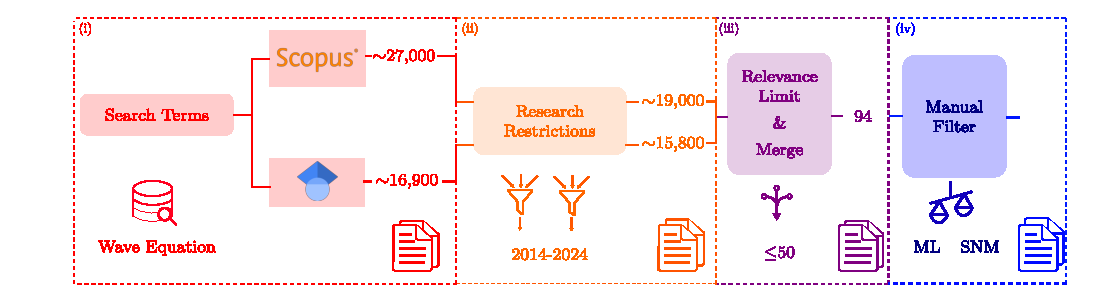
\includegraphics[width=1.0\textwidth]{figs/scheme_systematic_review.pdf}
\caption{Search flowchart and number of publications after each step. During the systematic review process, 
Scopus and Google Scholar were utilized with the relevant search terms (i), and the research was restricted to works 
in English and within the time frame of 2014-2024 (ii). The resulting lists were then sorted by relevance and limited 
to a maximum of 50 entries, with duplicates removed (iii). Finally (iv), a manual filter was applied by reading the 
titles and abstracts to ensure the publications were pertinent to our chosen field.}\label{fig:scheme_systematic_review}
\end{figure}

Initially, our search focused on how machine learning has been used for modeling wave propagation. The initial 
search was conducted using the following query on the Scopus and Google Scholar websites as an initial filter: 

\begin{quote}
\noindent\textbf{\texttt{"machine learning" OR "deep learning" OR "neural networks" AND "wave\linebreak
propagation" OR "wave equation" AND (modeling OR modelling OR model\linebreak
OR simulation)}}.
\end{quote}

The search was limited to articles published between 2014 and 2024, written in English. The resulting list was then 
sorted by relevance, with the analysis limited to the first 50 results from both 
databases, which were then merged, and duplicate works removed. The final list was manually filtered by 
reading the titles and abstracts, with relevance to the chosen field, which was computational seismology, 
as the inclusion criterion. Additionally, the list was restricted to works that provided a comparative 
analysis between machine learning methods and standard numerical methods in the abstract. 

The number of articles that passed the manual filtering process was \_. From these, we extracted relevant information to 
address the research question. The articles were summarized using on the following criterias: the application domain 
inside computational seismology, the machine learning method used, the standard numerical method with which it was 
compared and the reported main outcome from the comparison. In the case of physics-informed neural networks, 
the application domain their main outcome was also extracted. The Table \ref{tab:systematic_review} summarizes 
the main findings of the reviewed articles. 

From the resulted list of articles, we identified that the introduction of physics-informed neural 
networks has generated a large amount of work related. For example the work of 
\citeauthoryear{karimpouli_physics_2020} explores the application of deep learning in geosciences, 
specifically solving the 1-dimensional time-dependent seismic wave equation. Comparing Gaussian process 
and physics-informed neural networks, the research shows that these meshless methods, requiring 
smaller datasets, effectively incorporate physics laws, with the Gaussian process excelling in 
solution prediction and the neural network proving superior in velocity and density inversion. 
Their significant potential lies in addressing surrogate modeling and inverse analysis, 
striking a balance between accuracy and computational efficiency \citep{Song2022}. 
\citeauthoryear{rash_2022} took a similar  approach, but extending to 2D heterogeneous acoustic 
media, showing that PINNs could invert for ellipsoidal and checkerboard velocity models 
given the seismic response from sources placed within these models.

In \citeauthoryear{moseley_physics-informed_2022}, physics-informed neural networks were successfully 
applied to the 2D acoustic wave equation, demonstrating satisfactory outcomes in forward wave propagation and 
full waveform inversions, despite the efficiency of standard methods. Additionally, physics-informed neural networks 
showcased efficient performance in solving the inverse problem. To train the model, the results of a finite difference 
model are used. Spatial and temporal coordinates are used as inputs and intra-inputs of the network and their respective 
wave field as output, which provides uniqueness to the solution. While restricting the solution obtained to the equation 
used. To test the model, 3 different speed models are used: homogeneous, layered and an irregular model of the Earth's subsoil.

Similarly, in \citeauthoryear{ren_seismicnet_2024}, physics-informed neural networks were employed for modeling 
mechanical wave propagation in semi-infinite domains, showcasing their versatility in forward modeling for seismic 
wave propagation, without requiring labeled data. These studies collectively highlight the effectiveness of physics-informed 
neural networks across different wave propagation scenarios.

%--------------------------------------------------------------------------------------------------
% Section - Conclusions
%--------------------------------------------------------------------------------------------------
\section{Conclusions}\label{sec:conclusions}
\fancyhead[RO]{\textit{Conclusions}\, / \thepage}
%--------------------------------------------------------------------------------------------------

In this review, we have discussed the advancements in wave propagation modeling achieved through machine learning
methods, with a focus on computational seismology. We have provided an overview of the fundamentals of wave
propagation modeling, standard numerical methods, and the recent advances in machine learning methods to solve
differential equations. We have conducted a systematic review of the literature to identify the applications where
machine learning methods have demonstrated superior or comparable performance to standard numerical methods in terms
of computational time and accuracy. It is important to recognize that deep learning methods should complement, 
rather than replace, standard numerical techniques for solving partial differential equations. Traditional methods 
have been refined over decades to meet robustness and computational efficiency criteria in real-world applications. 
While this review focuses on computational seismology applications, the discussed methods can be applied to other 
fields where the wave equation is relevant. Future research should aim to integrate the strengths of both machine 
learning and traditional numerical methods, exploring hybrid approaches that can leverage the advantages of each 
technique.

%------------------------------------------------------------------------------------------------------------------------
% Import references from the bibliography file
%------------------------------------------------------------------------------------------------------------------------
\bibliography{refs}

\end{document}
%------------------------------------------------------------------------------------------------------------------------
% Document finish here
%------------------------------------------------------------------------------------------------------------------------